\section{Introduction}
Hardware performance counters are architecture-specific special-purpose registers integrated into modern CPUs, and can be used to profile applications.
As an example, modern Intel processors support hardware counters that report CPU utilization, L1 cache misses, branch mispredictions and a host of other CPU-specific performance indicators.
This information is invaluable when profiling low-level software performance.
What is more, compared to traditional software-based profiling, hardware performance counters incur negligible overhead because they are integrated into the hardware.
However, this performance advantage comes at a price.
Support for hardware counters is still in early stages, and requires linux kernels 2.6.31 or above.
There is still work to be done to make hardware counters trivial to use.
%Indeed, hardware performance counters are still nontrivial to use.

Tiptop~\cite{rohou:hal-00639173} is an application developed by Erven Rohou\footnote{\texttt{erven.rohou@inria.fr}} and is an attempt towards an intuitive interface for accessing hardware performance counters in modern CPUs.
The interface for tiptop is similar to the popular top\footnote{\texttt{\url{http://sourceforge.net/projects/unixtop/}}} utility. 
In tiptop's default configuration, it provides real-time statistics about running applications and their hardware performance counter values.
The values that appear on the real-time screen are configurable by the user and through use of an XML configuration file, multiple screens can be configured and flipped through in real-time.
In Figure~\ref{fig:tiptop-default} we have a screenshot of tiptop's default screen, and highlight a few of its key features.
The full breadth of hardware performance counters supported by tiptop are too many to list here, for a full list of features see the tiptop man page.

Despite the ease of use of tiptop, and its expansive set of hardware counters it supports via XML configuration, we identified a number of limitations.
In our initial investigation of tiptop we identified two bugs, we have confirmed these through personal communications with lead developer Erven Rohou.
Both bugs prevent tiptop from displaying statistics for processes.
For the first bug, we identified a solution that minimizes the probability that the bug occurs, and will work with Erven Rohou to include our patch into the main branch of the tiptop source.
The second bug remains unresolved, but can avoided by running tiptop as root, and we hope to identify a better solution for the final version of this project.

In addition to fixing existing bugs, we identified two feature enhancements for tiptop.
First, we now include the number of threads per-process as a column in the default tiptop screen, and also provided hooks to allow a user to specify the number of threads as a column in custom screens, via XML configuration.
Then, as a substantial feature enhancement, we have integrated the cross-platform Performance Application Programming Interface (PAPI)~\cite{Mucci99papi:a} library into tiptop.
%in order to simplify the process of developing XML files that work for tiptop across multiple platforms.
Integration with the PAPI library increases the breadth of platforms and kernel versions supported by tiptop, and simplifies the process of specifying XML configuration files that define custom tiptop screens.

In section~\ref{sec:methodology} we give an overview of our high-level development cycle and the tools we used to repair and enhance tiptop.
In section~\ref{sec:results} we give further details about the bugfixes and feature enhancements we identified for this project.
We conclude in section~\ref{sec:conclusion} with a discussion about additional feature improvements for future versions of tiptop.

\begin{figure}[t]
\footnotesize
\centering
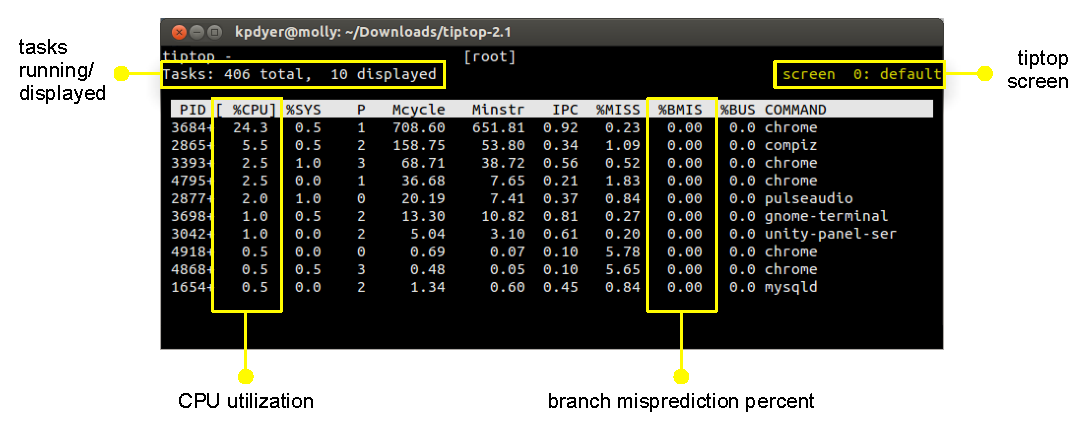
\includegraphics[width=1\textwidth]{tiptop-default}
%\hspace{.1in}
%\includegraphics[width=0.48\textwidth]{tiptop-default-screenshot-1}
\caption{A screenshot of the default screen for tiptop version 2.1. Each row in the display represents a single process.
In the top-left corner we have the number of running and displayed processes.
By default, tiptop only displays processes that have non-zero CPU utilization.
In the bottom-left we highlight the CPU utilization, reported as percentage of cycles used since the last screen refresh.
In the bottom-right corner we highlight the number of branch mispredictions.
Finally, in the top-right we highlight the label for the current screen.
Multiple views with custom columns can be configured and flipped through (using the right and left arrow keys) in real-time.}
\label{fig:tiptop-default}
\end{figure}